
\section{Versuchsaufbau}
\label{sec:Versuchsaufbau}

\begin{figure}
    \centering
    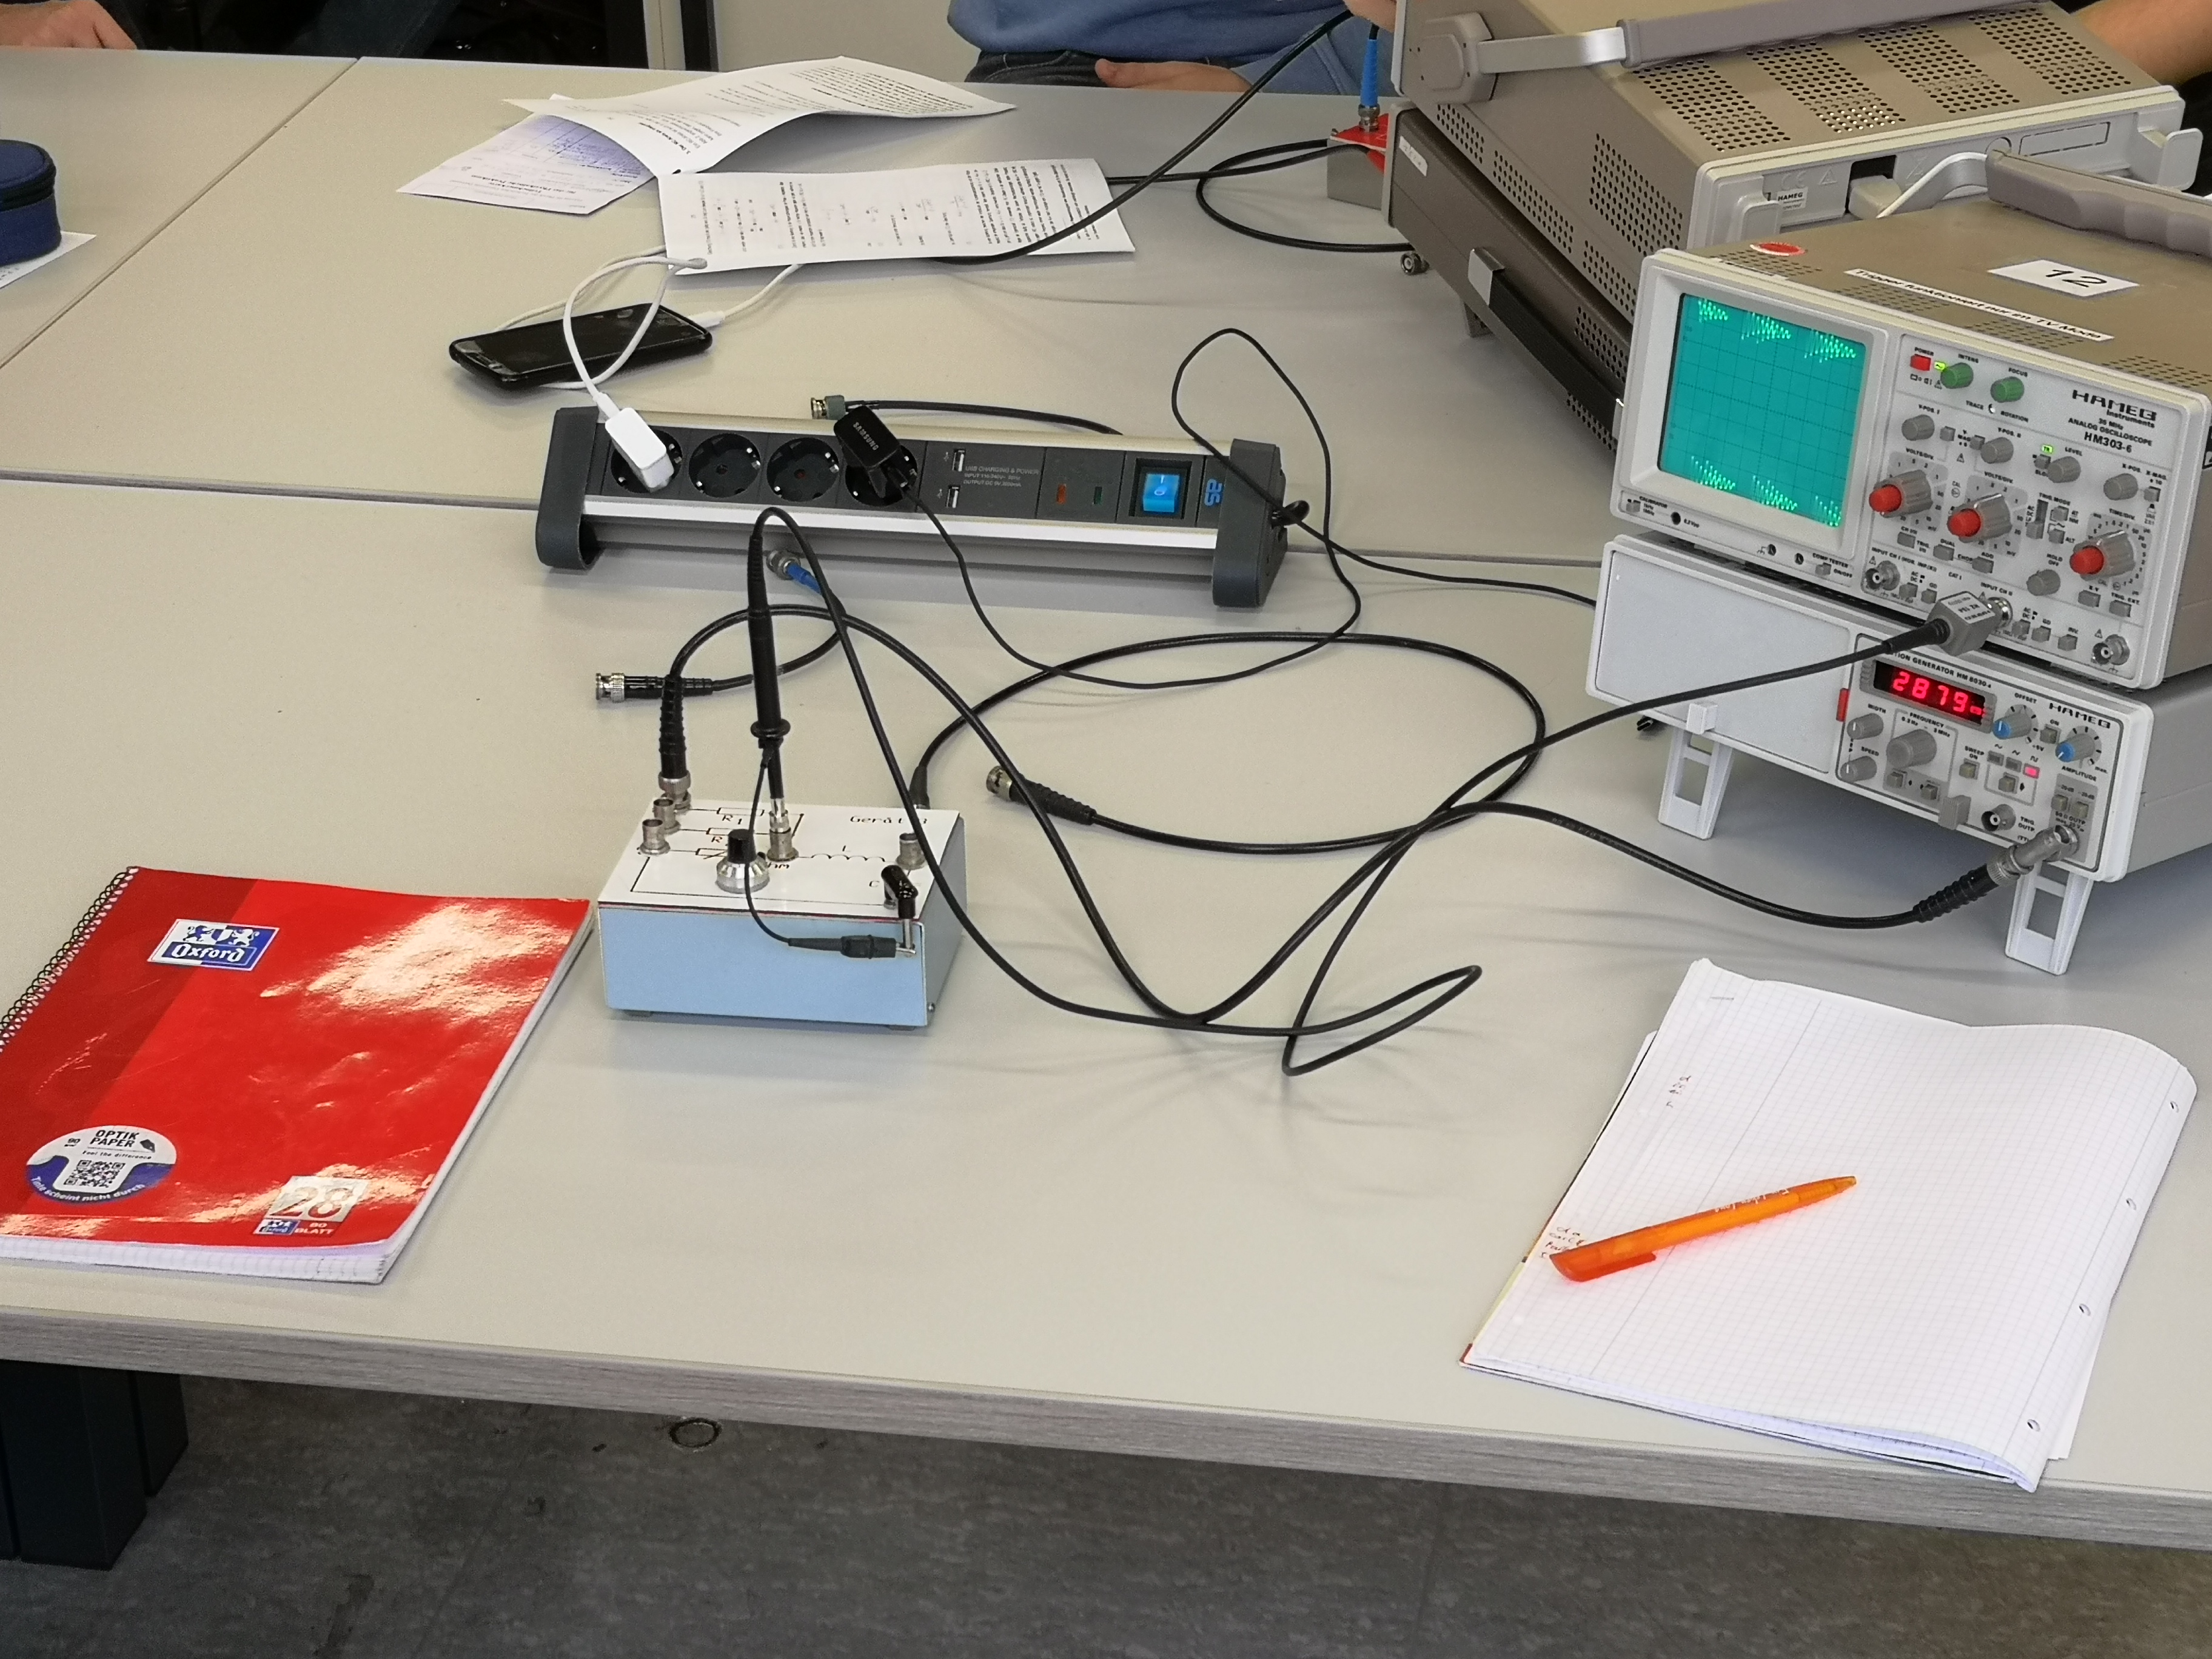
\includegraphics[width=0.8\textwidth]{content/Aufbau.jpg}
    \caption{Aufbau des Experiments.}
    \label{fig:aufex}

    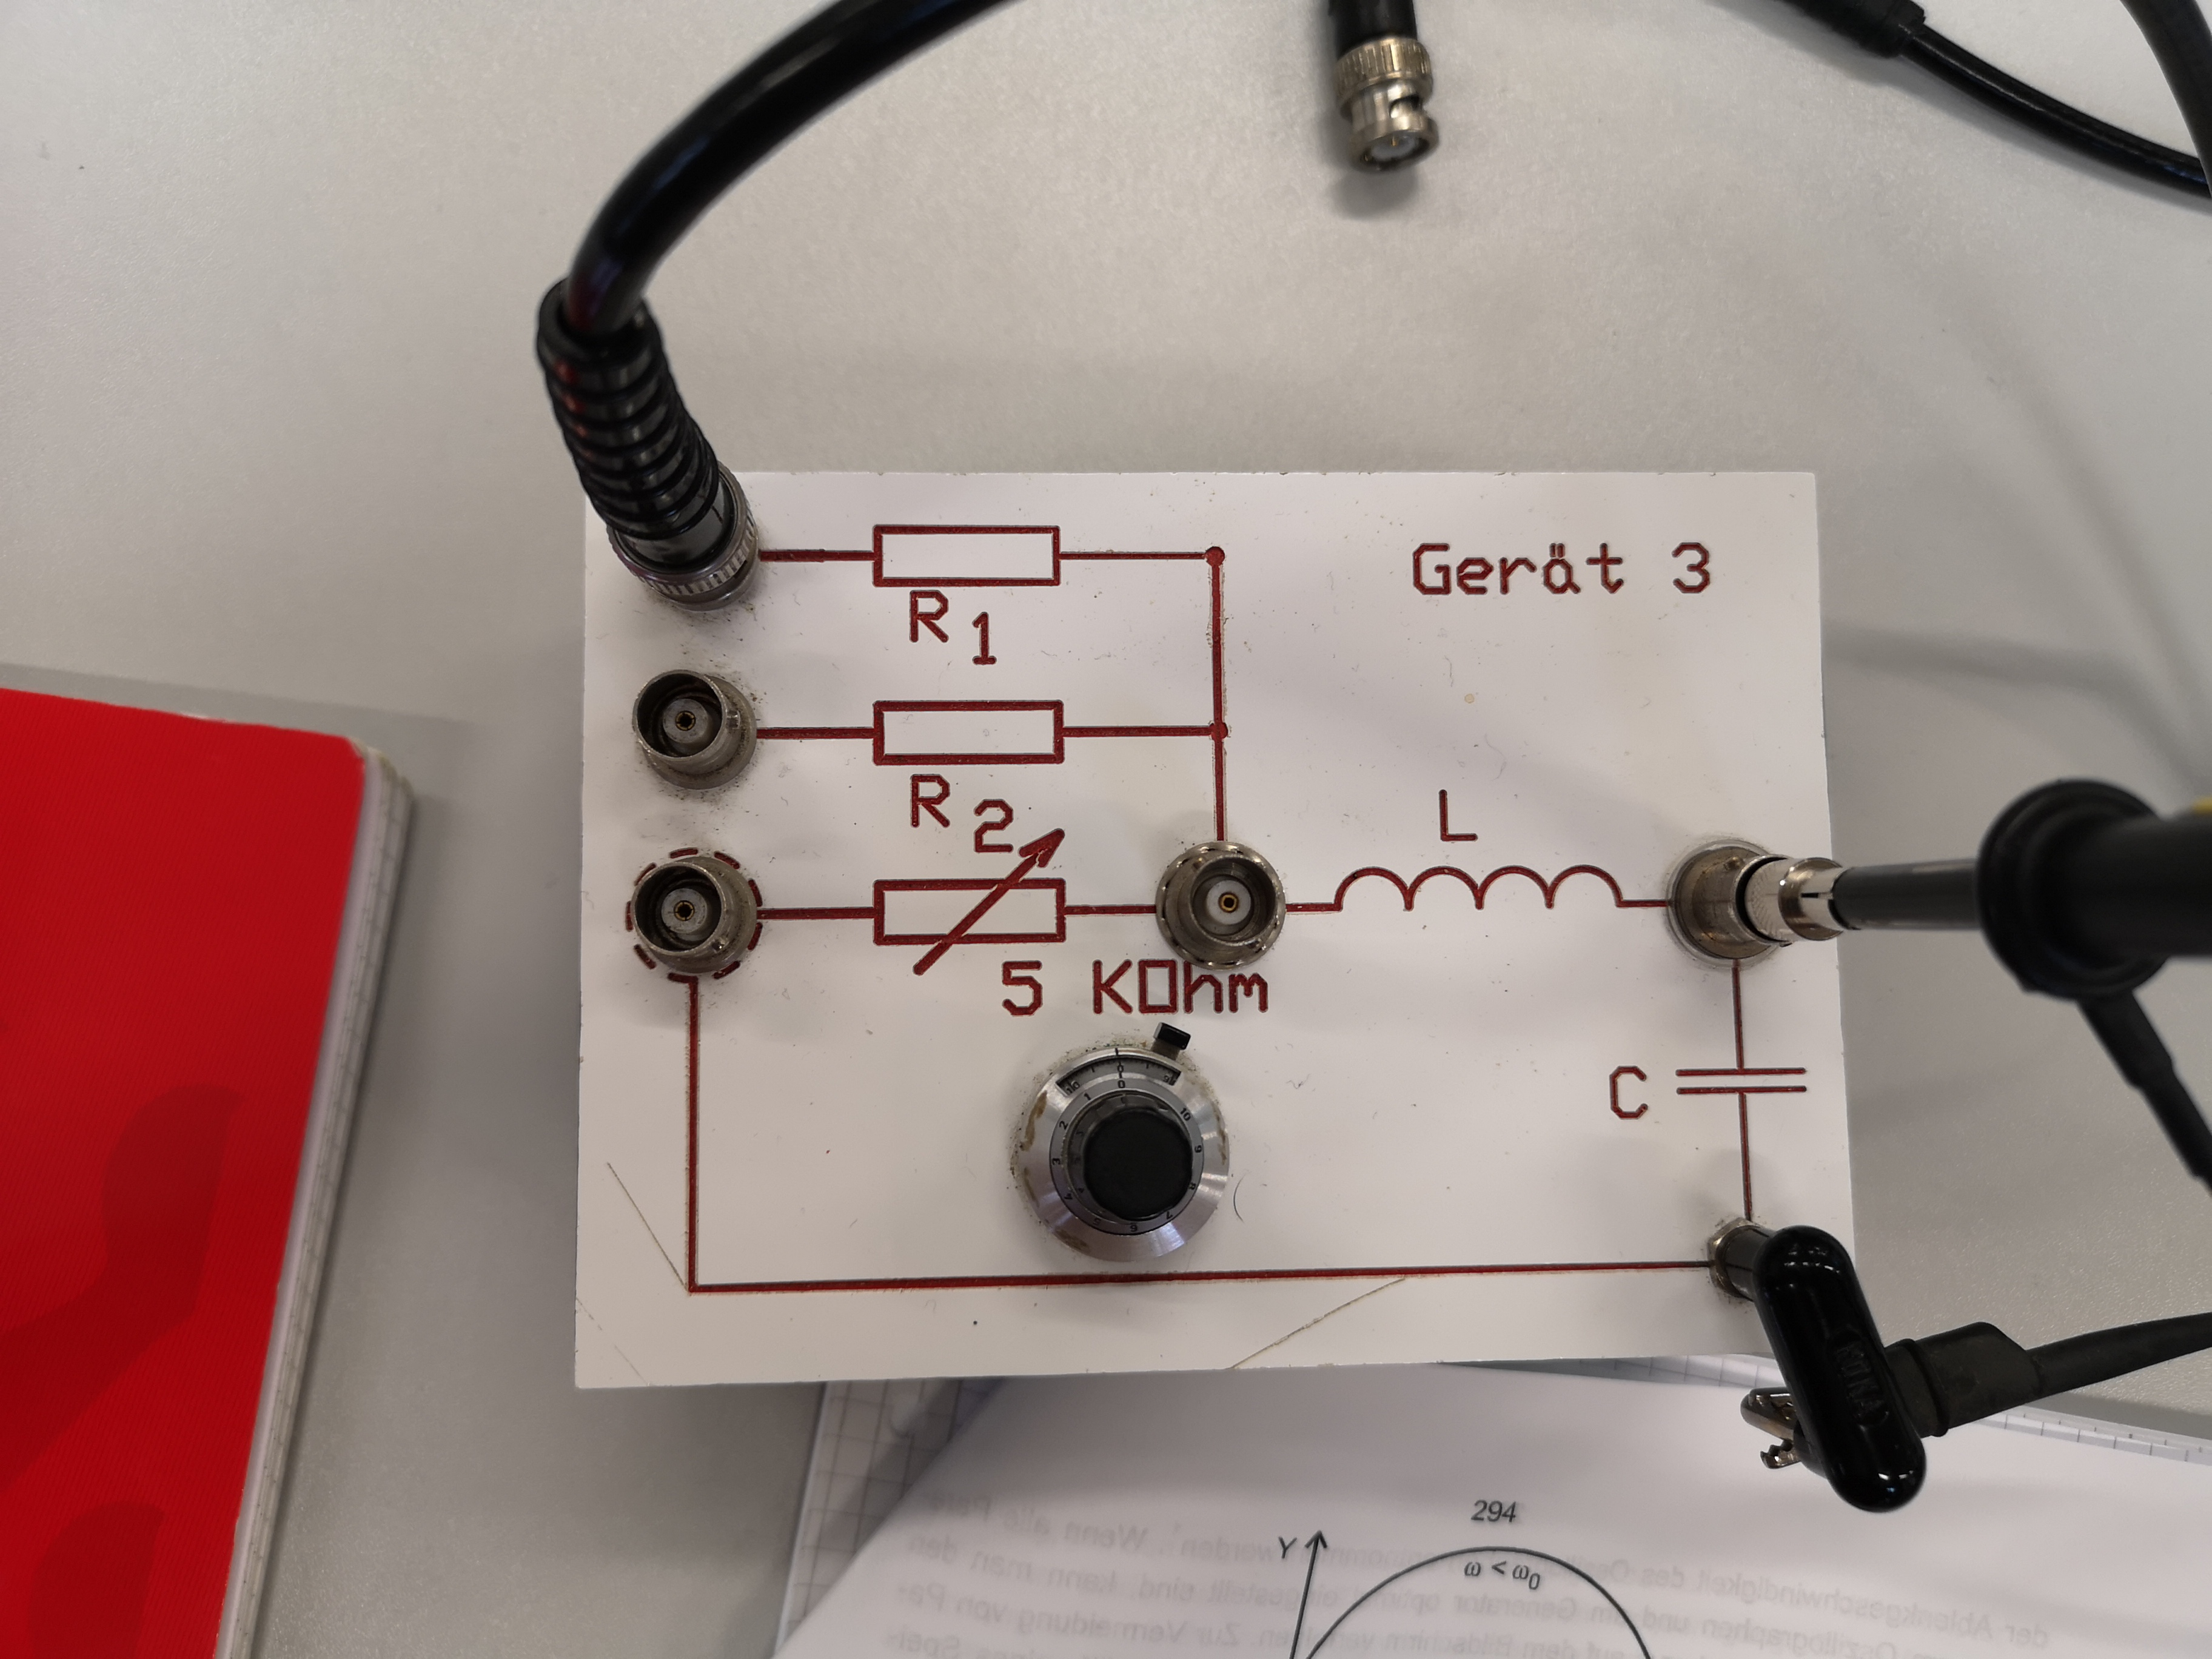
\includegraphics[width=0.8\textwidth]{content/Schaltkreis.jpg}
    \caption{Der Schaltkreis.}
    \label{fig:schalt}
\end{figure}
In \autoref{fig:aufex} und \autoref{fig:schalt} ist der grundsätzliche Aufbau zu sehen. 
Die Anschlüsse, sowie die eingestellten Werte variieren je nach Teilaspekten von \autoref{sec:Durchführung}.
